\section{Kinematics}
In order to control the UAV with regards to where the camera is pointing, a kinematic model that maps the camera focus to the UAV position and attitude is needed. The position of the UAV will be given in reference frame \{n\} using the North East Down (NED) coordinate frame:

\begin{equation}
	\bm{p}_{b/n}^n =
	\begin{bmatrix}
		N \\ E \\ D
	\end{bmatrix}
	=
	\begin{bmatrix}
		x_n \\ y_n \\ z_n
	\end{bmatrix}
\end{equation}

The attitude of the UAV will be given as Euler-angles:

\begin{equation}
	\bm{\Theta}_{nb} = 
	\begin{bmatrix}
		\phi \\ \theta \\ \psi
	\end{bmatrix}.
\end{equation}
	
These two expressions is often put together to make one position and orientation vector $\bm{\eta}$:

\begin{equation}
	\bm{\eta} =
	\begin{bmatrix}
		\bm{p}_{b/n}^n \\
		\bm{\Theta}_{nb}
	\end{bmatrix}.
\end{equation}
	
\subsection{Wind}
Wind will introduce what is called crab angle $\chi_c$ in the horizontal plane and the angle of attack $\gamma_a$ in the vertical plane. This will change the UAVs actual heading $\psi$ and pitch $\theta$ to \cite{suaBEARD}:

\begin{subequations}
\begin{equation}
	\chi = \psi + \chi_c
\end{equation}
\begin{equation}
	\gamma = \theta + \theta_a
\end{equation}
\end{subequations}

where $\chi$ is called the course and $\gamma$ is maybe called something??? These angles will only affect the navigational part, and not where the camera is pointed.


\subsection{Camera Position}

\begin{figure}
	\import{/}{kinematic_figure.tex}
	\caption{Illustration of how the angles influence the camera position.}
	\label{fig:camera_kinematics}
\end{figure}
	
The point where the camera is pointing is coupled with the attitude of the aircraft. Figure \ref{fig:camera_kinematics} shows how the position of the camera is affected by the attitude $\bm{\Theta}_{nb}$ in the body frame \{b\}, and the height $z_n$ in the NED frame \{n\}. This model assumes flat earth. The camera position in the body frame is expressed as

\begin{equation} \label{eq:camera_pos}
	\bm{c}_b^b =
	\begin{bmatrix}
		c_{x/b}^n \\
		c_{y/b}^n
	\end{bmatrix}
	=
	\begin{bmatrix}
		z_n sin(\theta) \\
		z_n sin(\phi)
	\end{bmatrix}.
\end{equation}

In order to express the camera position $\bm{c}_b^b$ in \{n\}, the heading $\psi$ of the aircraft must be taken into consideration. This is done by rotating the point $\bm{c}_b^b$ with the rotational matrix $\bm{R}_{z,\psi}$:

\begin{equation} \label{eq:body_ned_rotate}
	\bm{c}_b^n =
	\begin{bmatrix}
		c_{x/b}^n \\
		c_{y/b}^n
	\end{bmatrix}
	= \bm{R}_{z,\psi} \bm{c}_b^b,
\end{equation}

where:

\begin{equation}
	\bm{R}_{z,\psi} = 
	\begin{bmatrix}
		cos(\theta) & -sin(\theta) & 0 \\
		sin(\theta) & cos(\theta) & 0 \\
		0 & 0 & 1
	\end{bmatrix}.
\end{equation}

The point $\bm{c}_b^n$ is not the actual position in \{n\} since it does not take the UAVs position into consideration. This is done by simply adding the UAVs position to $\bm{c}_b^n$:

\begin{equation} \label{eq:body_ned_trans}
	\bm{c}^n =
	\begin{bmatrix}
		c_x^n \\ c_y^n
	\end{bmatrix}
	=
	\begin{bmatrix}
		x_n + c_{x/b}^n \\
		y_n + c_{y/b}^n
	\end{bmatrix}.
\end{equation}

\subsection{Camera Angle of View}
Since the camera isn't only focusing on one specific point, it can be useful describing the camera point of focus as two extremities instead of one center point. Equation \eqref{eq:camera_pos} can easily be changed to do this. Assuming the camera has an angle of view $\sigma$, the equation now becomes:

\begin{equation}
	\bm{e}_{1,b}^b = 
	\begin{bmatrix}
		e^b_{x/b} \\ e^b_{y_1/b}
	\end{bmatrix}
	=
	\begin{bmatrix}
		z_n sin(\theta)\\
		z_n sin(\phi + \sigma)
	\end{bmatrix}
	, \hspace{5pt}
	\bm{e}_{2,b}^b = 
	\begin{bmatrix}
		e^b_{x/b} \\ e^b_{y_2/b}
	\end{bmatrix}
	=
	\begin{bmatrix}
		z_n sin(\theta)\\
		z_n sin(\phi - \sigma)
	\end{bmatrix}.
\end{equation}

The steps for translating the points to the NED frame are the same as in \eqref{eq:body_ned_rotate} and \eqref{eq:body_ned_trans}:

\begin{equation}
	\bm{e}_b^n =
	\begin{bmatrix}
		e^n_{x/b} \\ e^n_{y/b}
	\end{bmatrix}
	= \bm{R}_{z,\psi} \bm{e}_b^b
\end{equation}

\begin{equation}
	\bm{e}^n =
	\begin{bmatrix}
		e^n_{x} \\ e^n_{y}
	\end{bmatrix}
	=
	\begin{bmatrix}
		x_n + e^n_{x/b} \\
		y_n + e^n_{y/b} \\
	\end{bmatrix}.
\end{equation}

\begin{figure}[!ht]
    \centering
    \makebox[\textwidth][c]{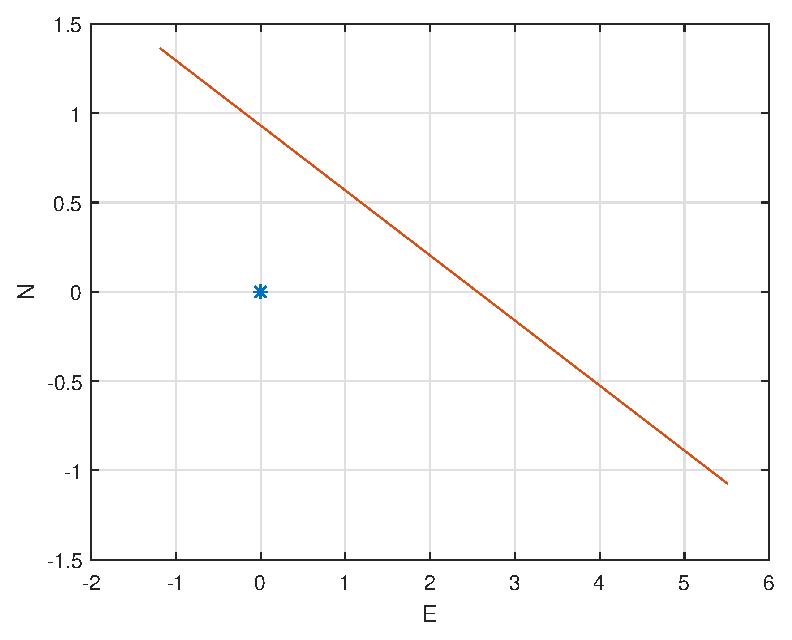
\includegraphics[width=1.25\textwidth, keepaspectratio=true]{../../trials/kinematic_output.eps}}
    \caption{Graph showing the line the camera captures when the plane is positioned in the origin with an altitude of $10m$, and $\phi=-10$, $\theta=-5$ and $\psi=20$. The field of view is $20\degree$.}
\end{figure}